The previous subchapter revealed that the proposed system of the designed environment, its state presentation, and the usage of behavioral cloning did not produce feasible predictions. Our established definition of "good" predictions and desired goal is 300 meters in average distance to the ground-truth, while the best setup achieved a median value for all trajectories of 707 meters and an average of 2136 meters (shown in Tab. \ref{tab:rlResults1}). The question arises, if this poor performance is due to behavioral cloning not being a suitable method or a misunderstanding at our side, e.g., the wrong modelling of the environment. In this subchapter, we will have a closer look at the state representation and reevaluate if the proposed environment truly fulfills the Markov property. We then expand the feature space and conduct another set of experiments, showing a significant improvement.
\par
Defined by Eq. \ref{eq:realStateRepresentation}, the current state definition includes the position of the vessel, as well as the direction and speed at a given time step $t$. Although, the internal policy network of behavioral cloning is trained with all possible state-action pairs in order to learn the underlying distribution of states to actions, the actual path prediction of the agent only depends on the initial state $s_0$. Whereas the policy network is in theory capable of memorizing different motion clusters, which start at the same position, the agent is not. Next predictions of the agent solely depend on the corresponding previous states, hence the whole trajectory gets generated based on the initial state. For the overall environment to be Markov, this initial state has to include all information necessary to distinguish between different ship routes and locations to go. In its current form, the state representation is insufficient because if two ships with the same speed and direction enter the observation window, the agent is unable to guess whether one of those two ships is going to enter the harbor or follow the Weser.
\par
Recalling from the discussion of chapter \ref{chap:synthetic}, the state representation has to be informative enough to represent the current snapshot of the environment at a certain time step. When following the advice given in subchapter \ref{subchap:nature} and taking an abstract look at the problem and the situation from the view of a captain, we can argue that the destination is present in the head of the captain at all times. Our assumption is, that adding additional information about the destination of the ship is crucial for the system to be Markov and even be usable in the reinforcement learning framework. To this extent, we add the angle and the distance from the current agent position to the destination. As already mentioned in subchapter \ref{chap:ais}, the destination attribute has to be manually set to be included in an AIS message. Additionally, our raw AIS dataset does not include the information of destination. For those reasons, we computed the destination by simply taking the last position of each trajectory. The resulting state representation is defined by:
\begin{equation}
    S3 := S_t = \{lon_t,lat_t, direction_t, speed_t, angle_t, distance_t\}
\end{equation}
\newpage
The conducted experiments shown in the upcoming Tab. \ref{tab:improvedTab} are done with a learning rate of $\alpha=1e^{-5}$, a batch size of 256 and an environment setup formulized as $S3\_A2$. The median, median absolute deviation (MAD) and mean are calculated in meters. As in the previous subchapter, we also include the histogram of trajectory performances from the best experiment run in Fig. \ref{fig:improvedHisto}.

\begin{table}[H]
\centering
\begin{tabular}{|l|l|l|l|l|l|}
\hline
\textbf{Dataset} & \textbf{Network}      & \textbf{Epochs} & \textbf{Median} & \textbf{MAD} & \textbf{Mean}   \\ \hline
Tanker           & $[512-256-128-64-32]$ & $30$            & $777$           & $571$        & $1402 \pm 1482$ \\ \hline
Big Ships        & $[512-256-128-64-32]$ & $30$            & $433$           & $240$        & $891 \pm 1135$  \\ \hline
Big Ships        & $[16-16]$             & $30$            & $459$           & $328$        & $1705 \pm 2262$ \\ \hline
Big Ships        & $[256-128-64]$        & $100$           & $419$           & $297$        & $2331 \pm 3954$ \\ \hline
\end{tabular}
\caption{}
\label{tab:improvedTab}
\end{table}


\begin{figure}[H]
         \centering
         \includesvg[width=0.7\textwidth]{images/ais/bar_plots/big_ships_S3_improved.svg}
       \caption{Histogram of trajectory performances, including information about the destination to the state representation $S3$. "Big ships" dataset with a network architecture of $n_h^1=512, n_h^2=256, n_h^3=128, n_h^4=64,$ and $n_h^5=32$.}
        \label{fig:improvedHisto}
\end{figure}

The Tab. \ref{tab:improvedTab} reveals a significant improved compared to the results sampled in the previous subchapter and a state representation without information about the destination. We again see, that the "big ships"-dataset is better suited as a training set due to the amount of given trajectories to train on, even though the "tanker"-dataset includes more similar trajectories that are very smooth. The best run utilizes a more complex network of 5 hidden layers and achieves a median of 433 meters as average distance across all trajectories (down from 707 meters). Even the biased value for the total mean decreased from 2136 down to 891 meters.
\par
The presented results allow for the conclusion that the previous environment was indeed not suitable to be applied to behavior cloning and not the other way around. Adding two additional features that include information of the destination makes the agent able to distinguish between different motion clusters.\newpage
This can also be seen by looking at concrete predictions, as illustrated in the upcoming Fig. \ref{fig:predictionsRL}:

\begin{figure}[H]
     \centering
     \begin{subfigure}[b]{0.48\textwidth}
         \centering
             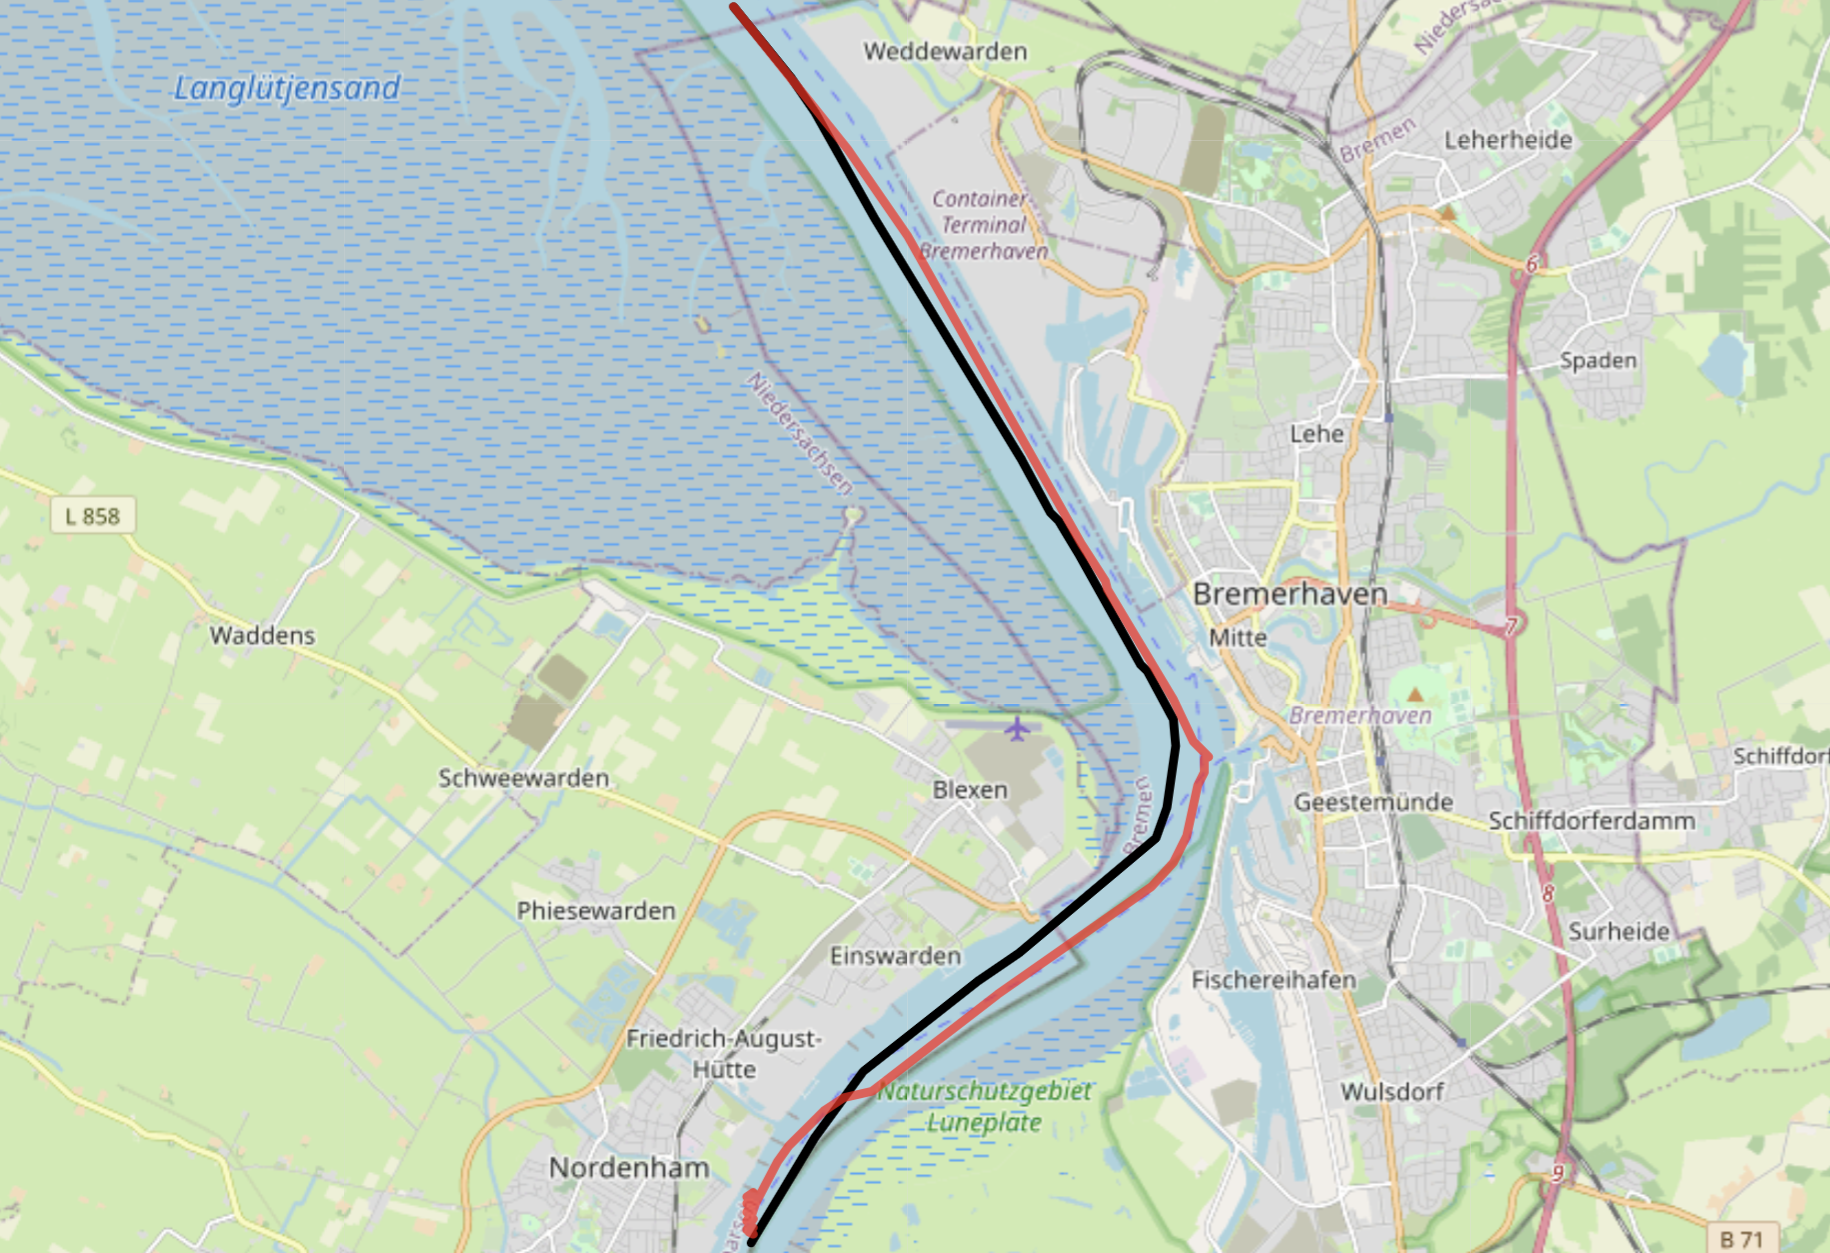
\includegraphics[width=\textwidth]{images/ais/tracks/pred1.png}
             \caption{}
         \label{fig:double3}
     \end{subfigure}
          \hfill
               \begin{subfigure}[b]{0.48\textwidth}
         \centering
             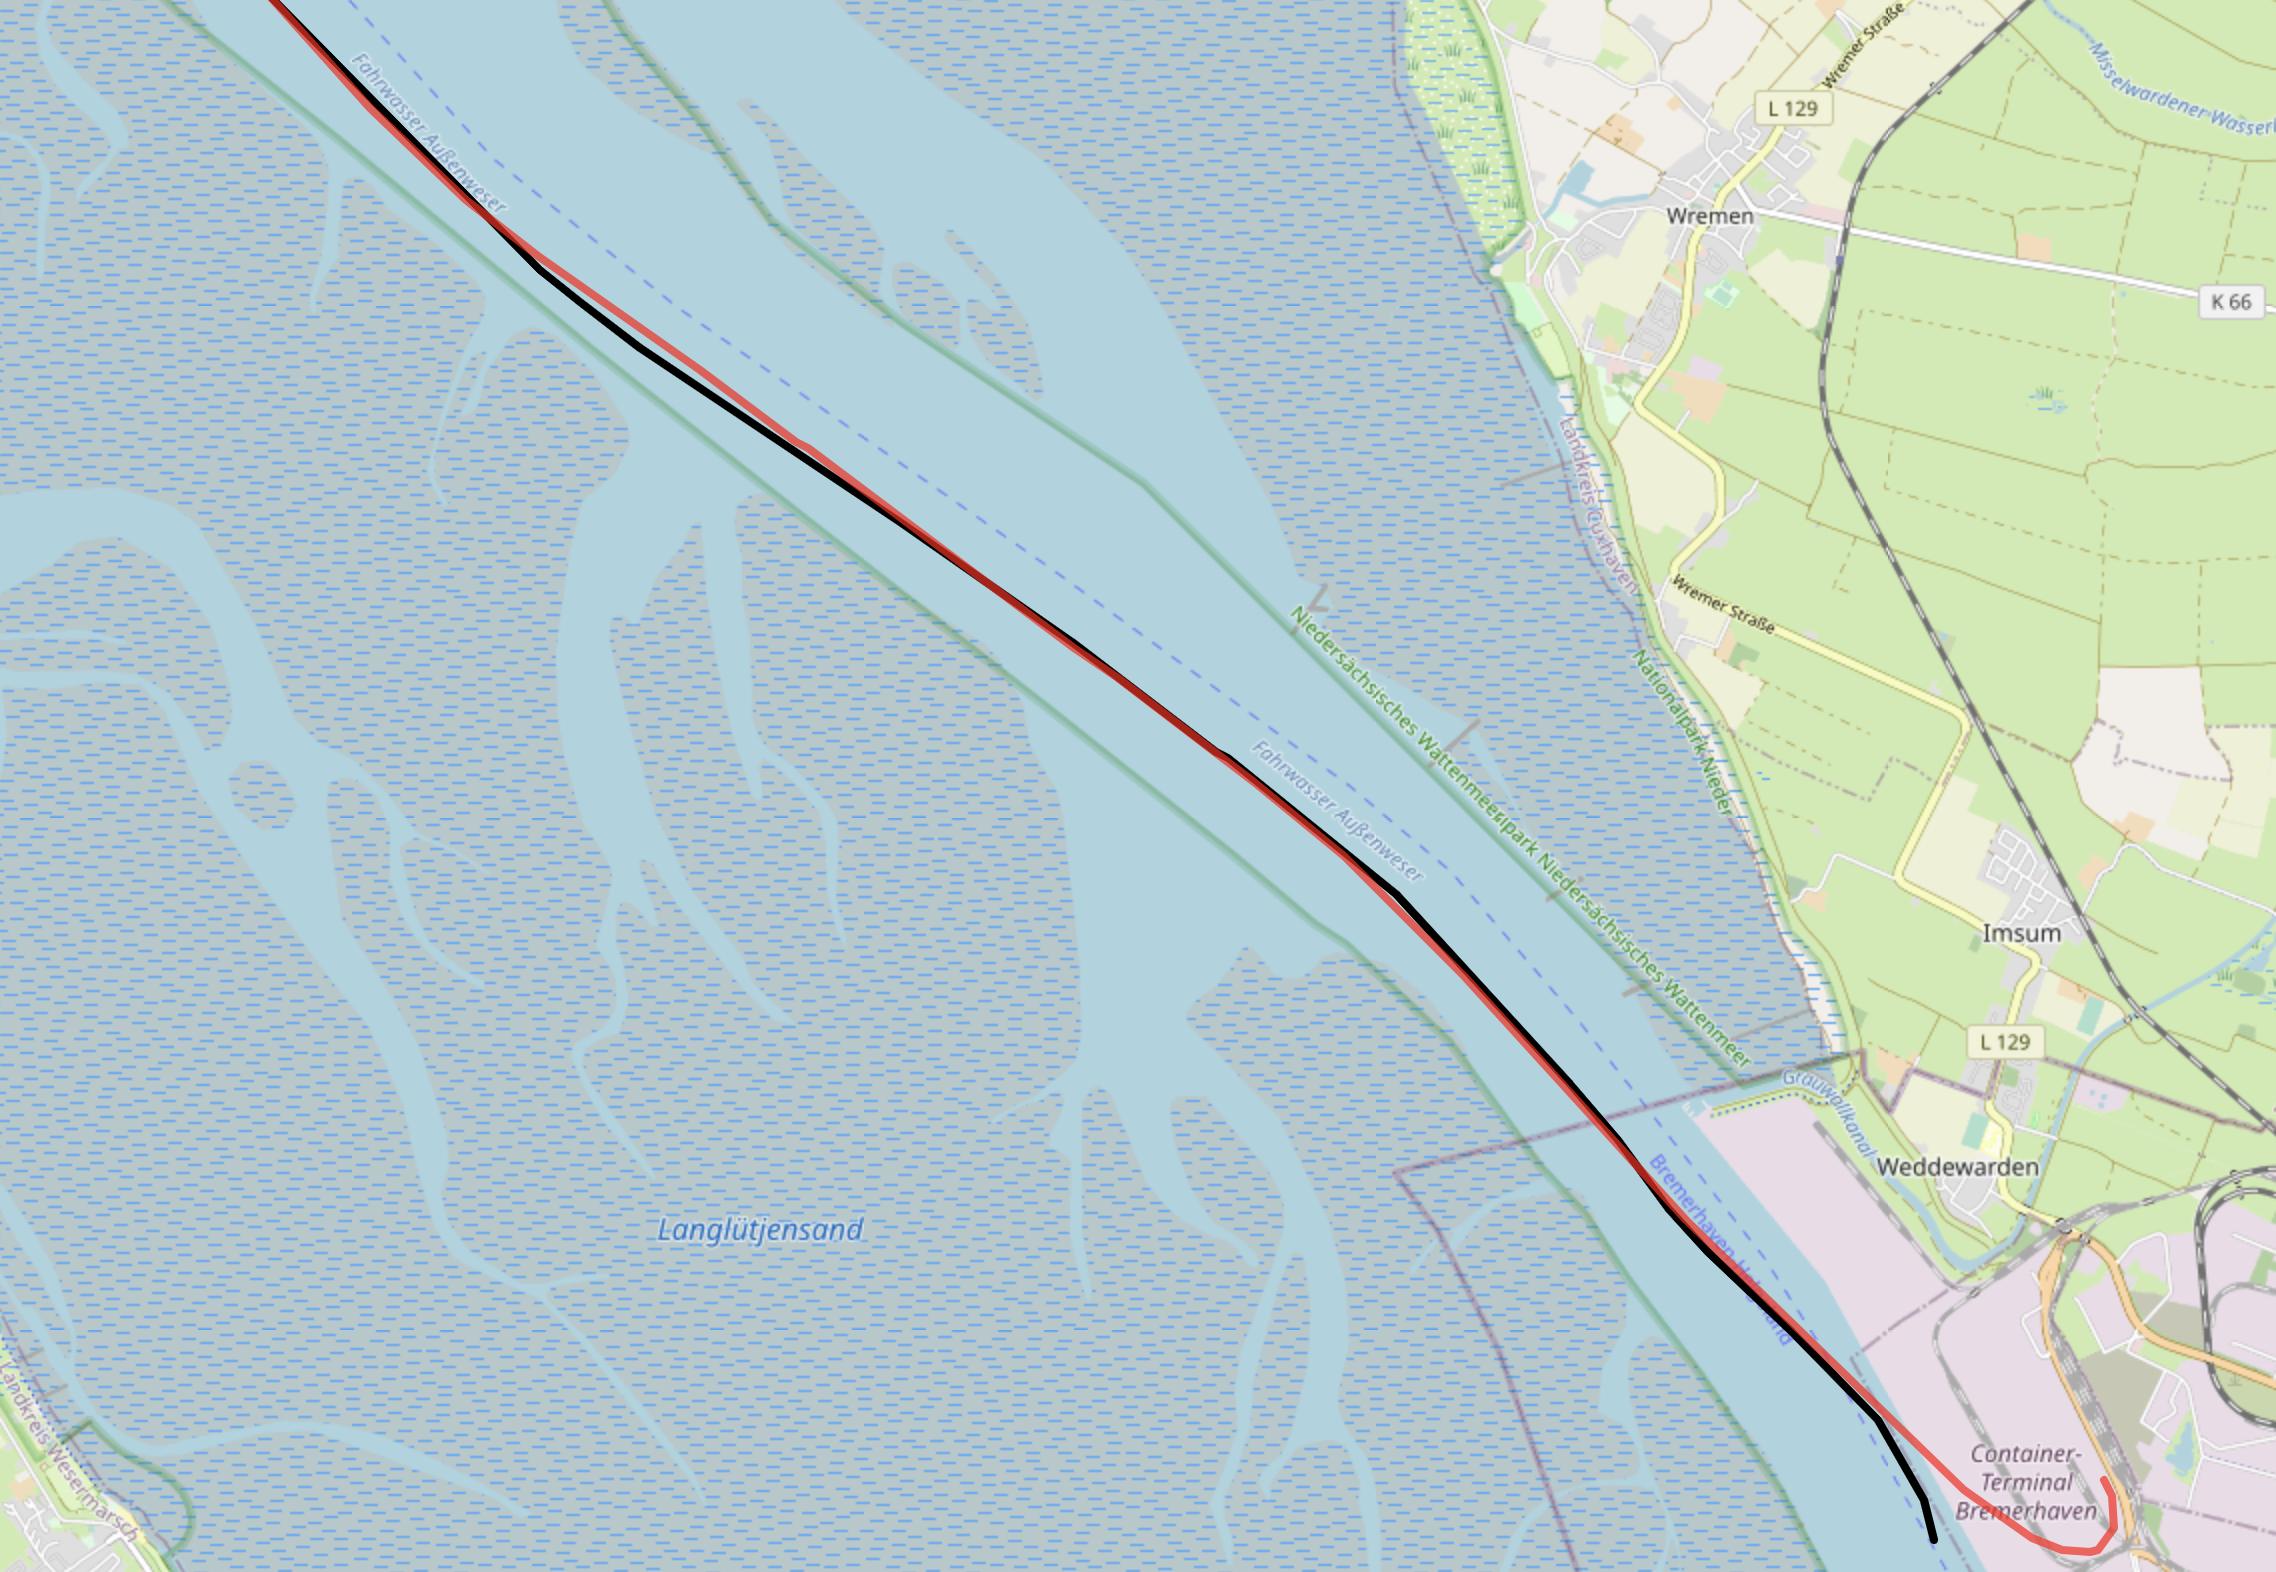
\includegraphics[width=\textwidth]{images/ais/tracks/pred7.png}
              \caption{}
         \label{fig:double4}
     \end{subfigure}
\end{figure}
\begin{figure}[H]\ContinuedFloat
     \begin{subfigure}[b]{0.48\textwidth}
         \centering
       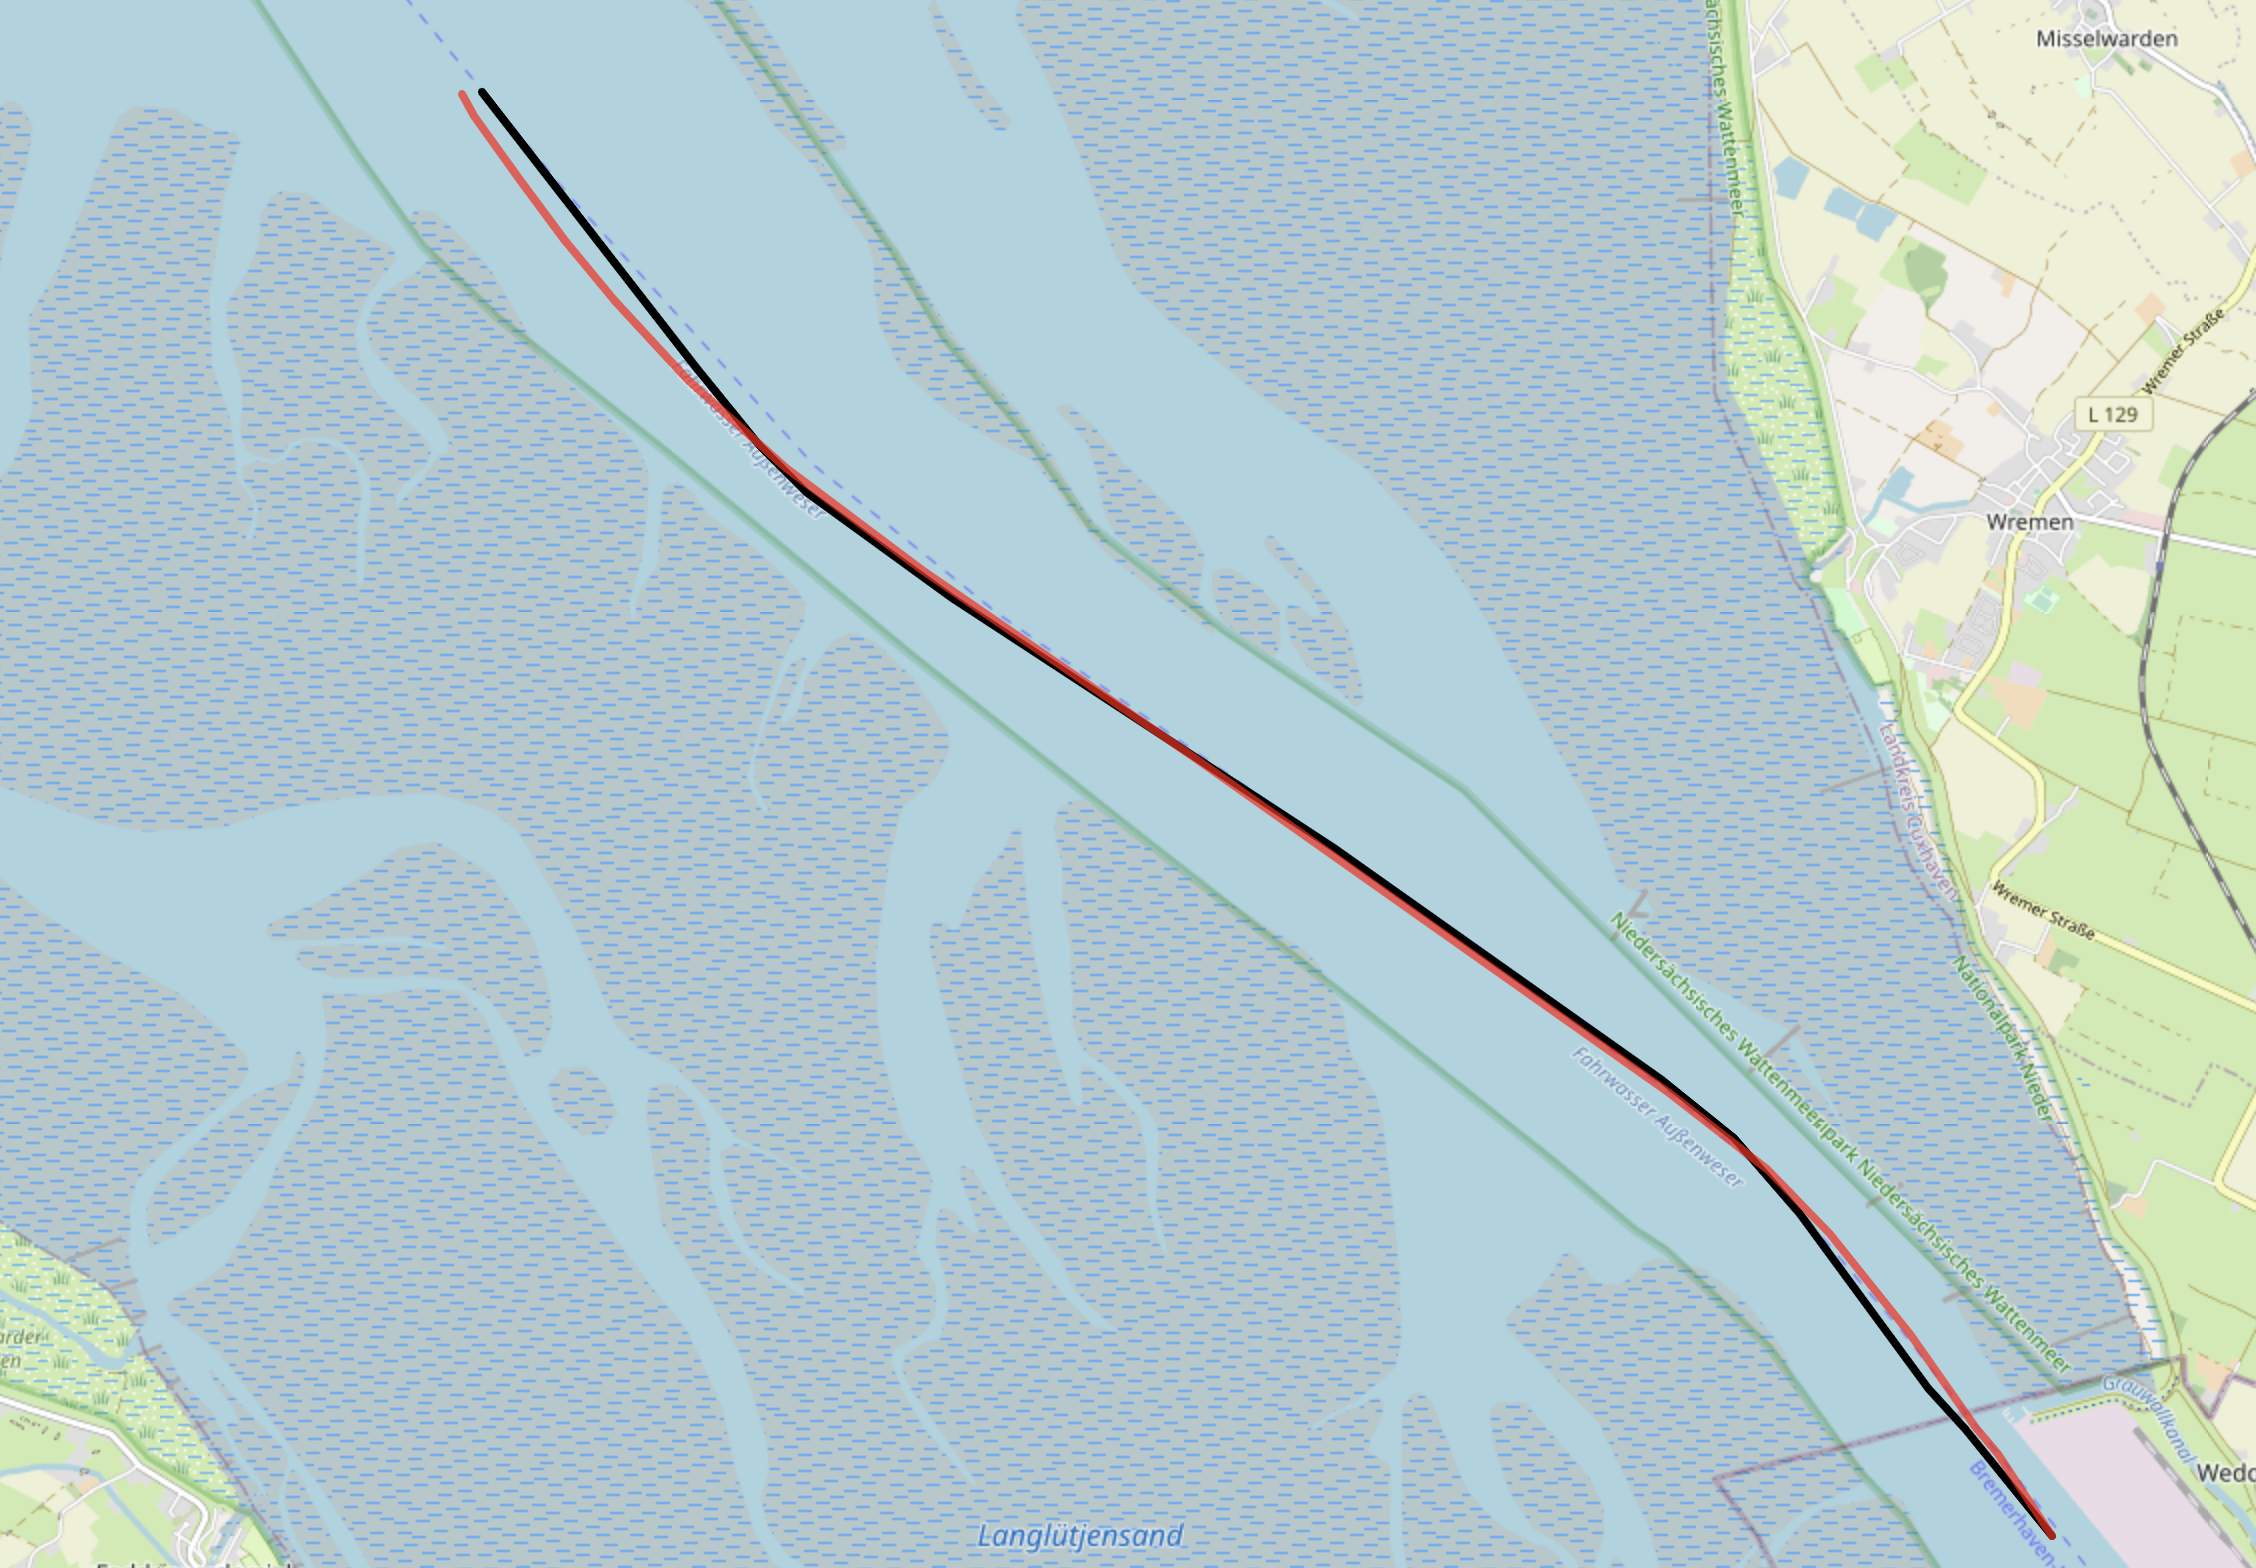
\includegraphics[width=\textwidth]{images/ais/tracks/pred3.png}
        \caption{}
         \label{fig:double1}
     \end{subfigure}
     \hfill
     \begin{subfigure}[b]{0.48\textwidth}
         \centering
             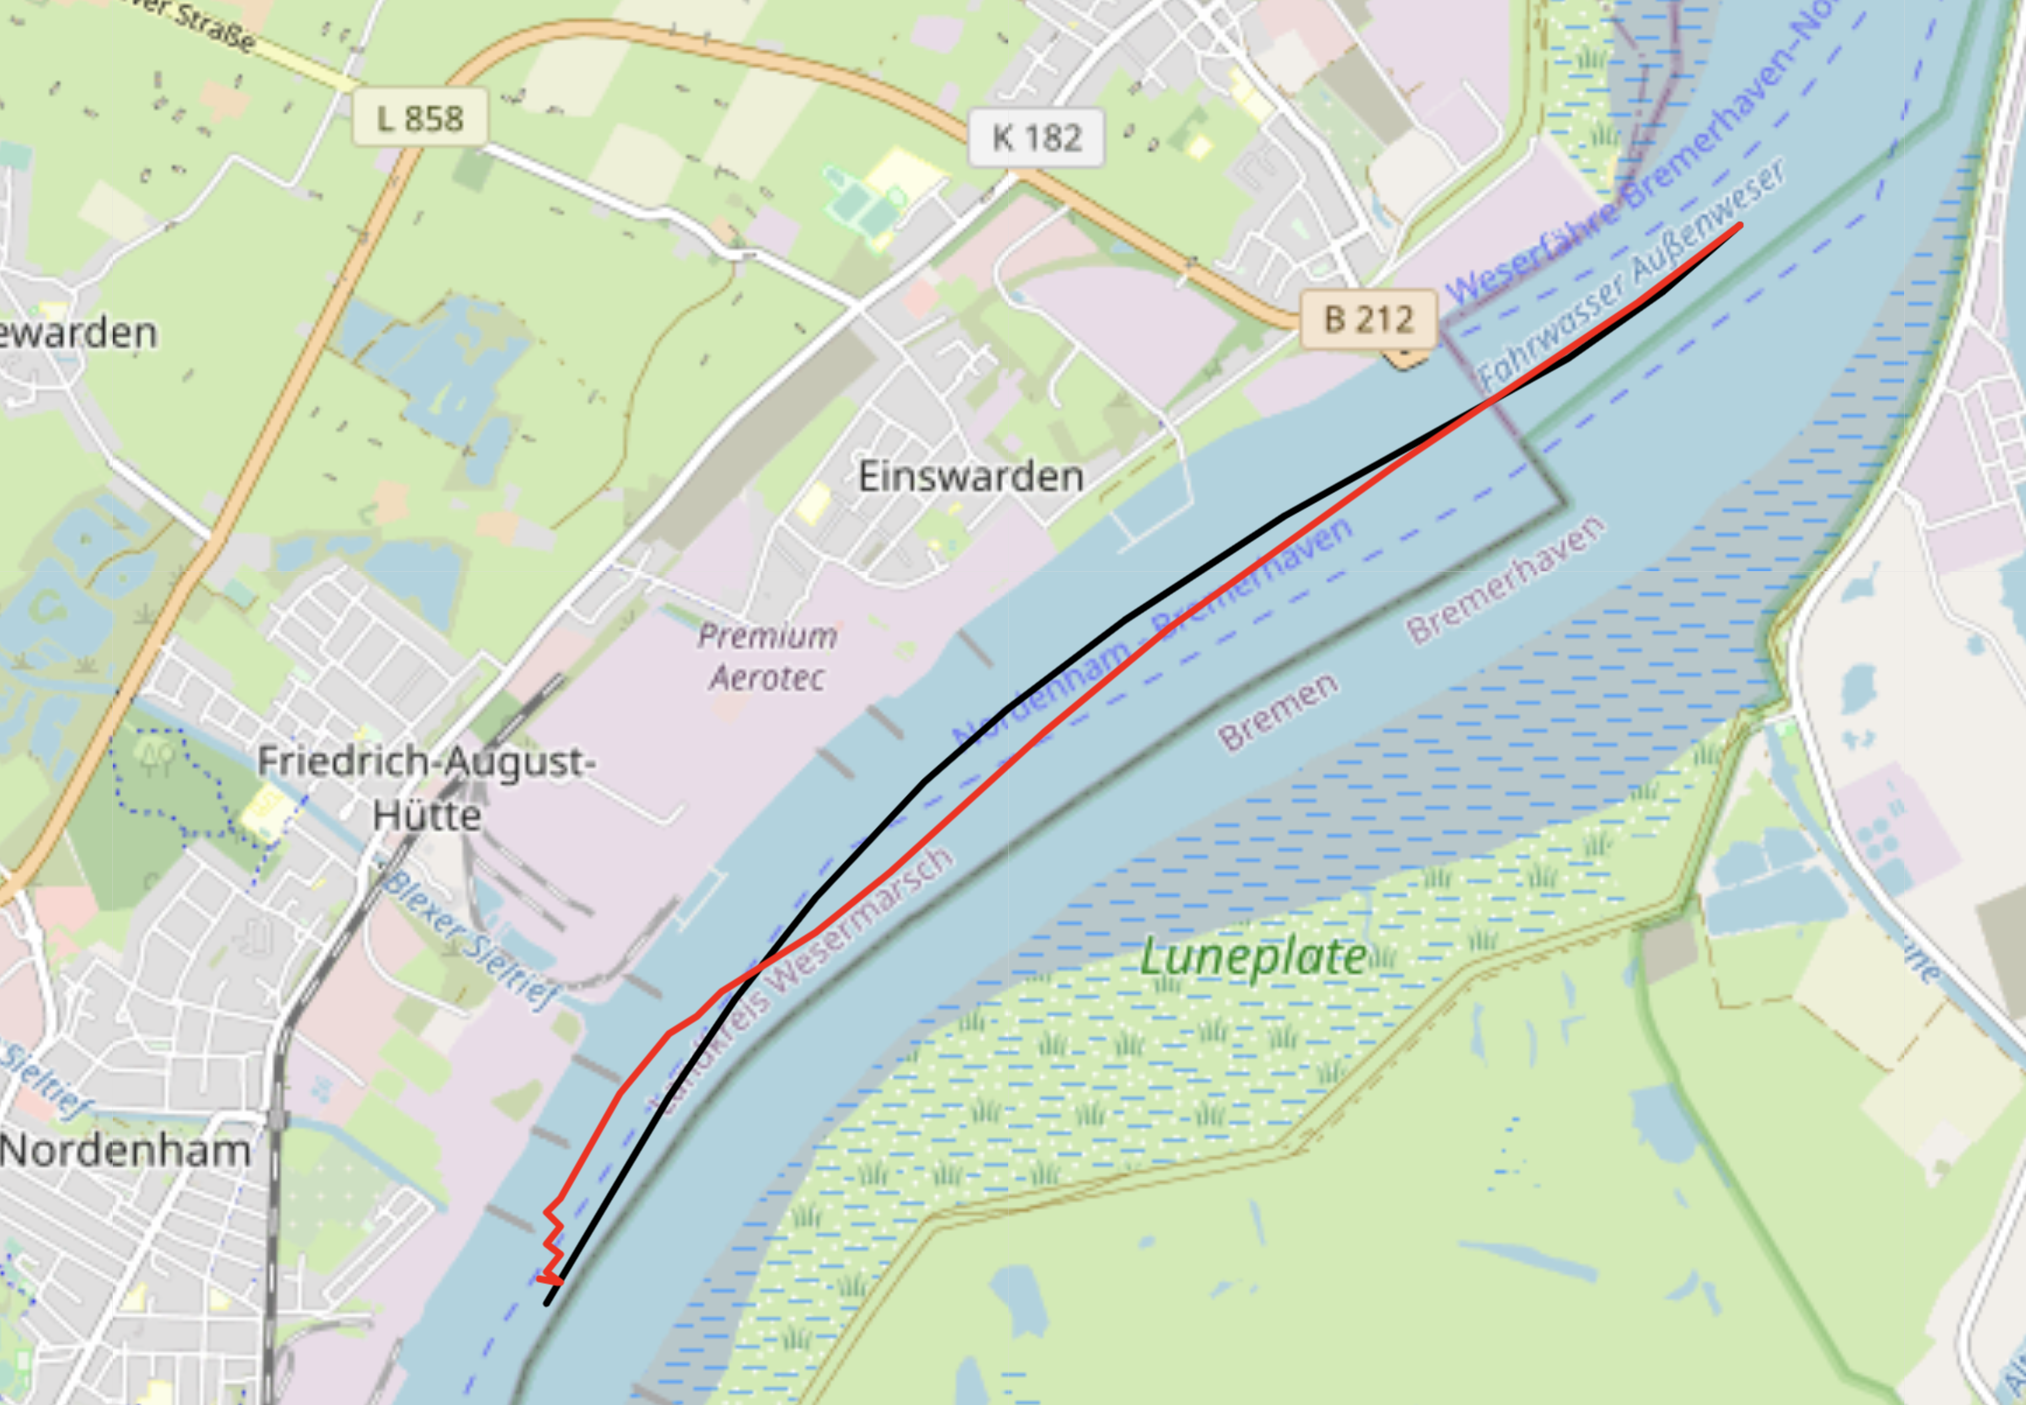
\includegraphics[width=\textwidth]{images/ais/tracks/pred2.png}
              \caption{}
         \label{fig:double2}
     \end{subfigure}
\end{figure}
\begin{figure}[H]\ContinuedFloat
     \begin{subfigure}[b]{0.48\textwidth}
         \centering
             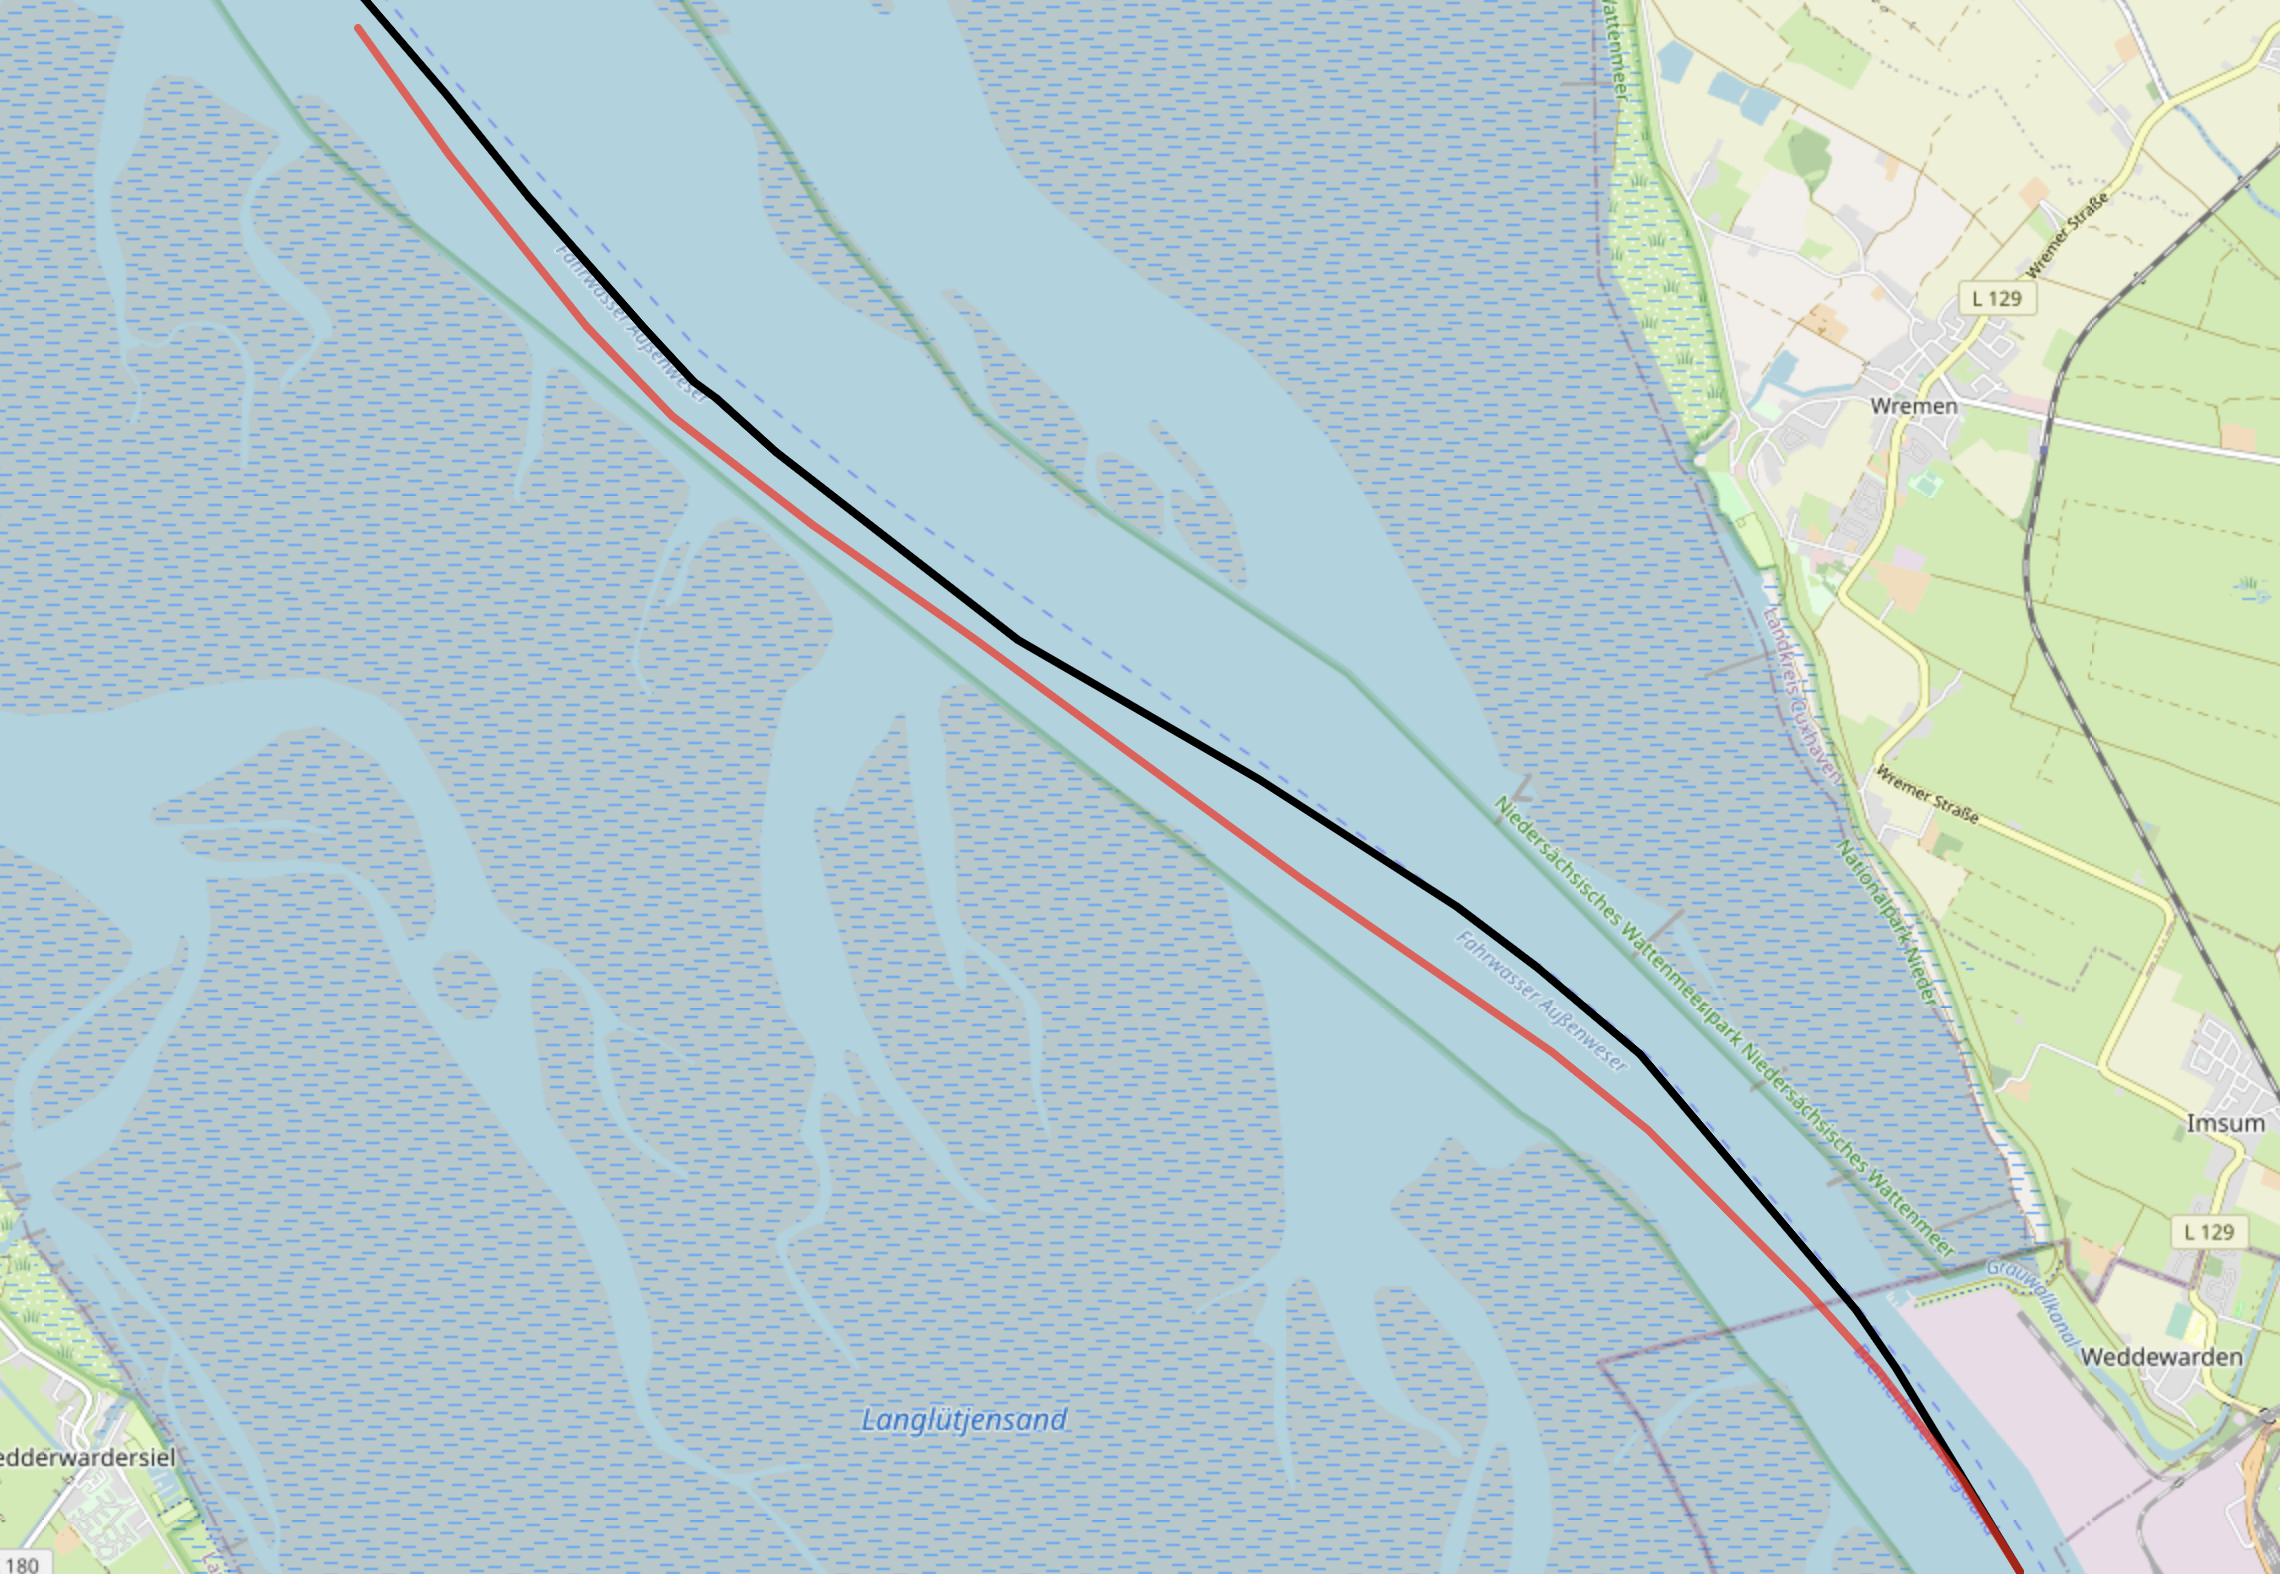
\includegraphics[width=\textwidth]{images/ais/tracks/pred5.png}
              \caption{}
         \label{fig:double5}
     \end{subfigure}
               \hfill
     \begin{subfigure}[b]{0.48\textwidth}
         \centering
             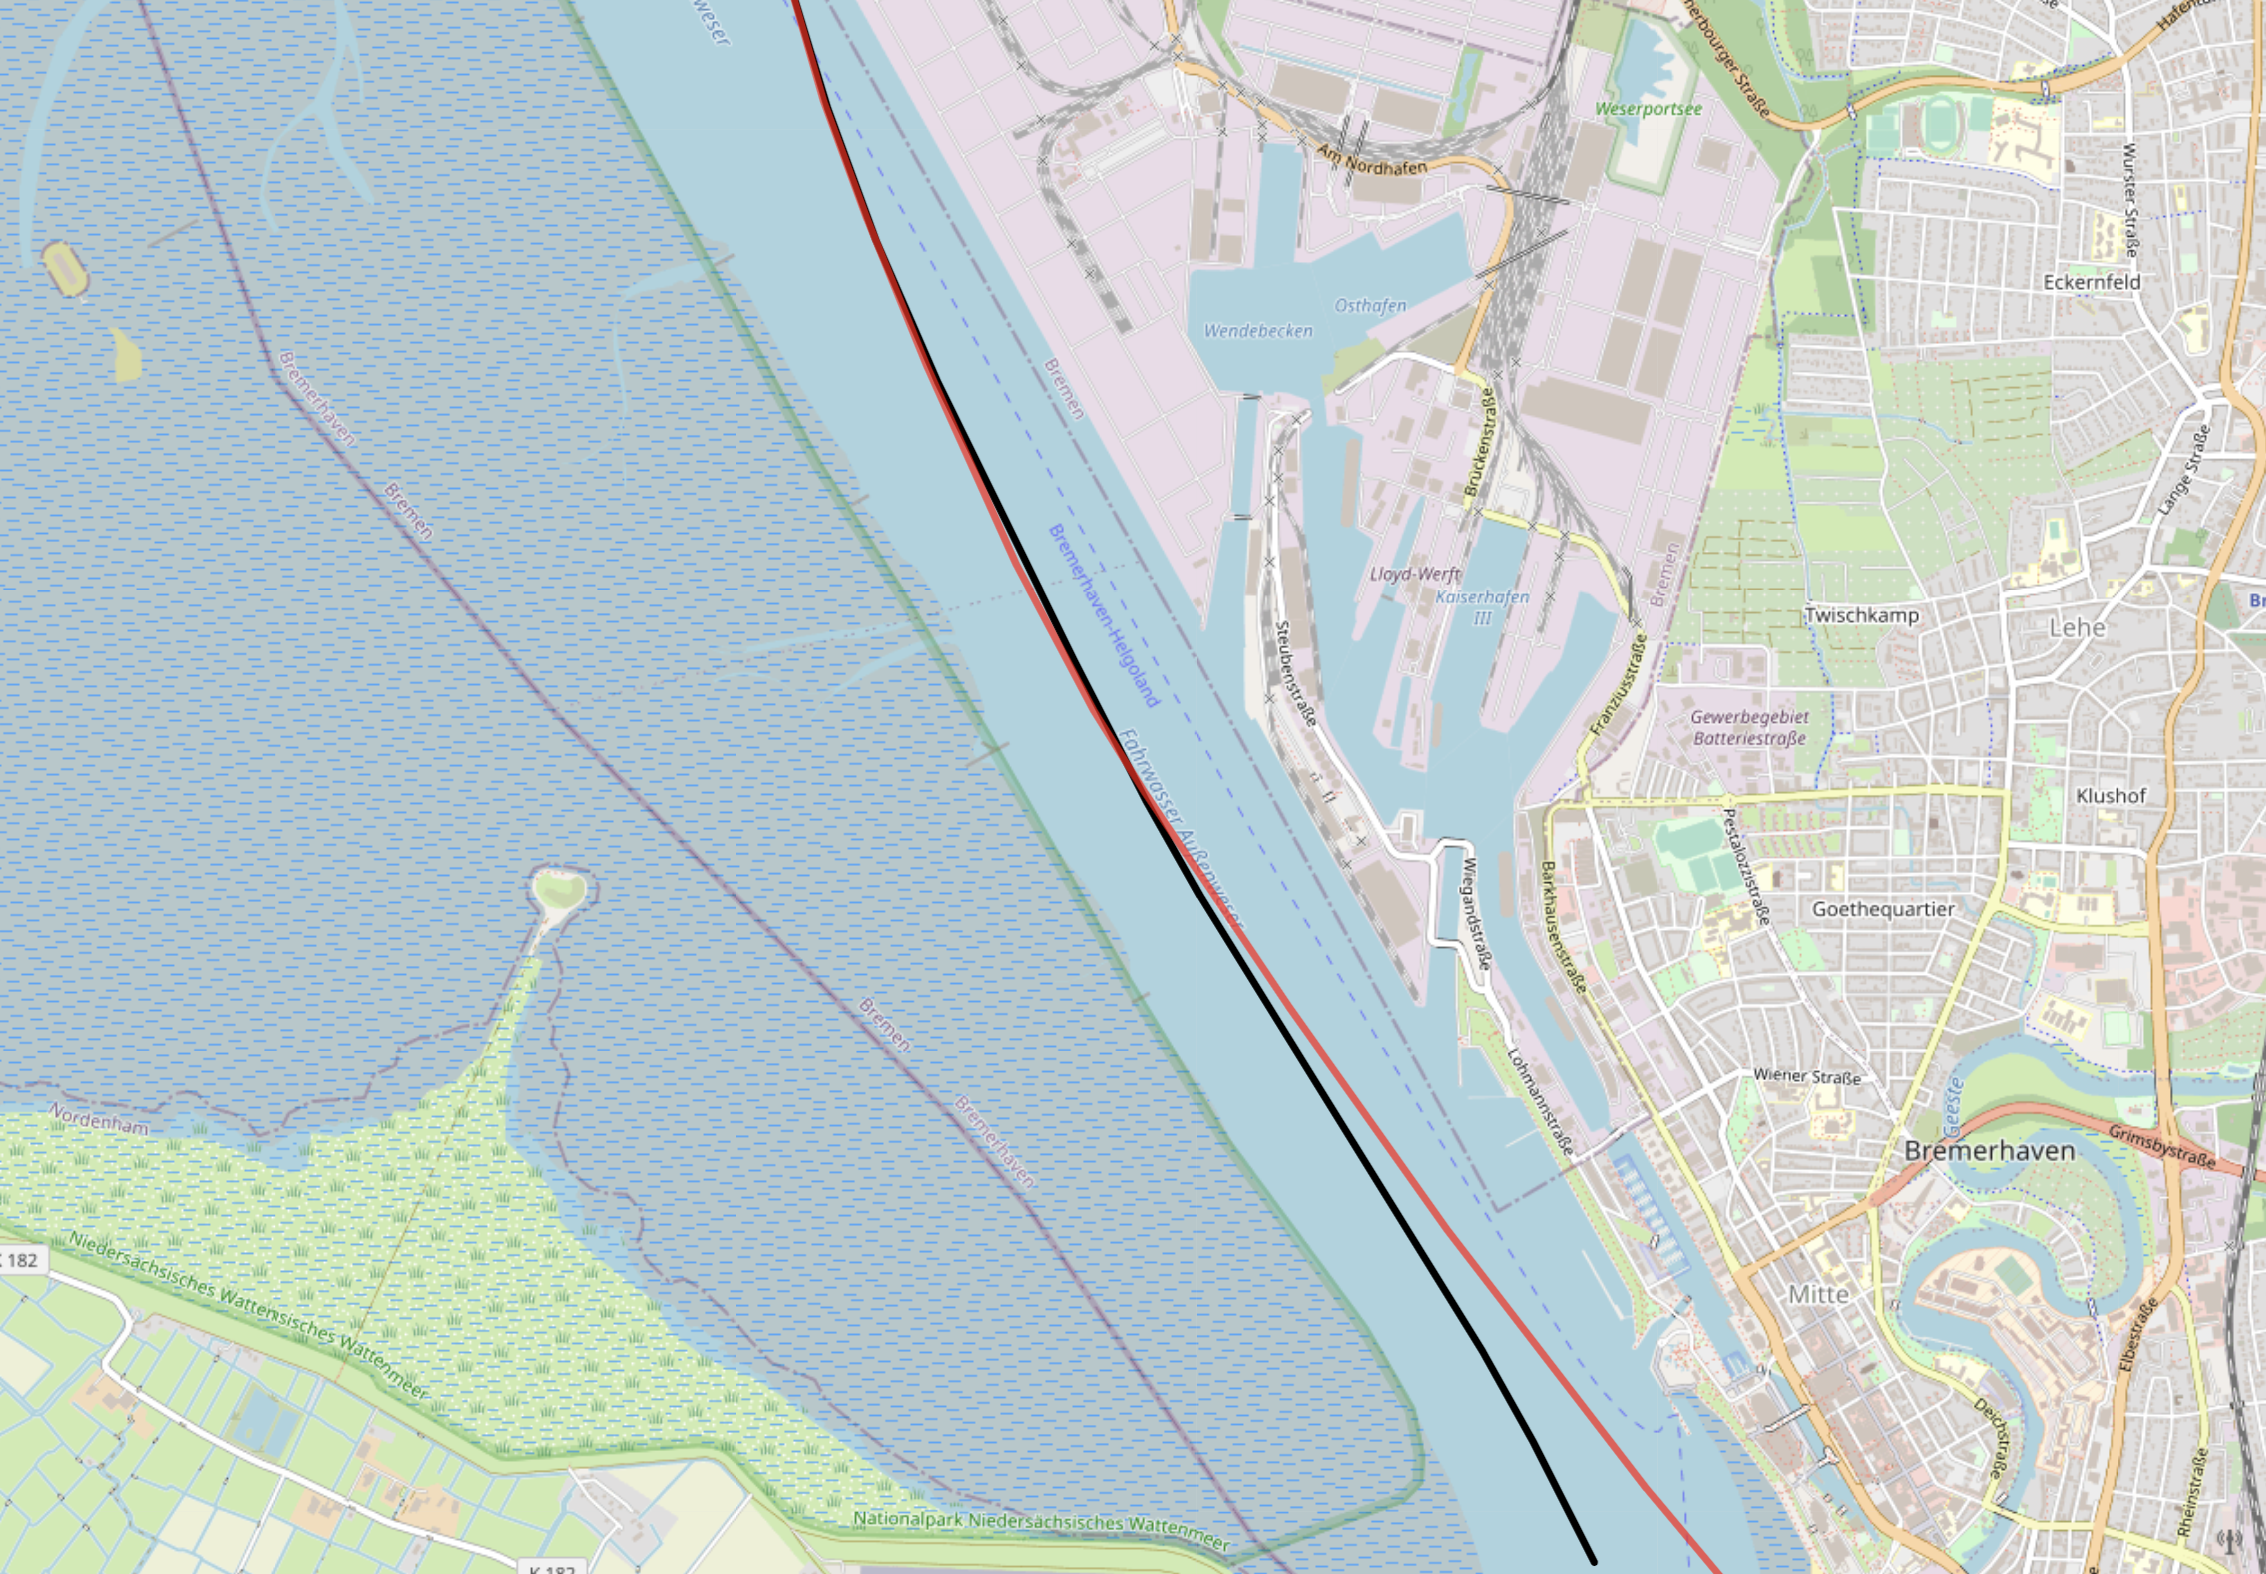
\includegraphics[width=\textwidth]{images/ais/tracks/pred6.png}
              \caption{}
         \label{fig:double6}
     \end{subfigure}
     \caption{Example predictions generated by the agent purely based on the initial state $s_0$ given by the test data. Red indicates the agent's path and black the ground-truth trajectory.}
     \label{fig:predictionsRL}
\end{figure}
